
\subsection{Programación variador de velocidad}


Para realizar la configuración del variador de velocidad con los parámetros del motor se utilizó el software SoMove a través del protocolo ModBus. Se descargó la ultima versión desde la página oficial de Schneider\footnote{\url{https://www.se.com/ar/es/product-range-presentation/2714-somove/}} y luego, la librería DTM correspondiente al variador a utilizado \footnote{\url{https://www.se.com/ar/es/download/document/Altivar_DTM_Library/}}.

Una vez realizado esto se procedió a generar un nuevo proyecto donde se eligió las características del variador (Figura \ref{fig:so1} y \ref{fig:so2}). El próximo paso fue realizar por medio del software la carga de los parámetros del motor (Figura \ref{fig:paramsomove}) y establecer el modo de funcionamiento de las entradas y el protocolo de comunicación.
\begin{figure}[h]
	\centering
	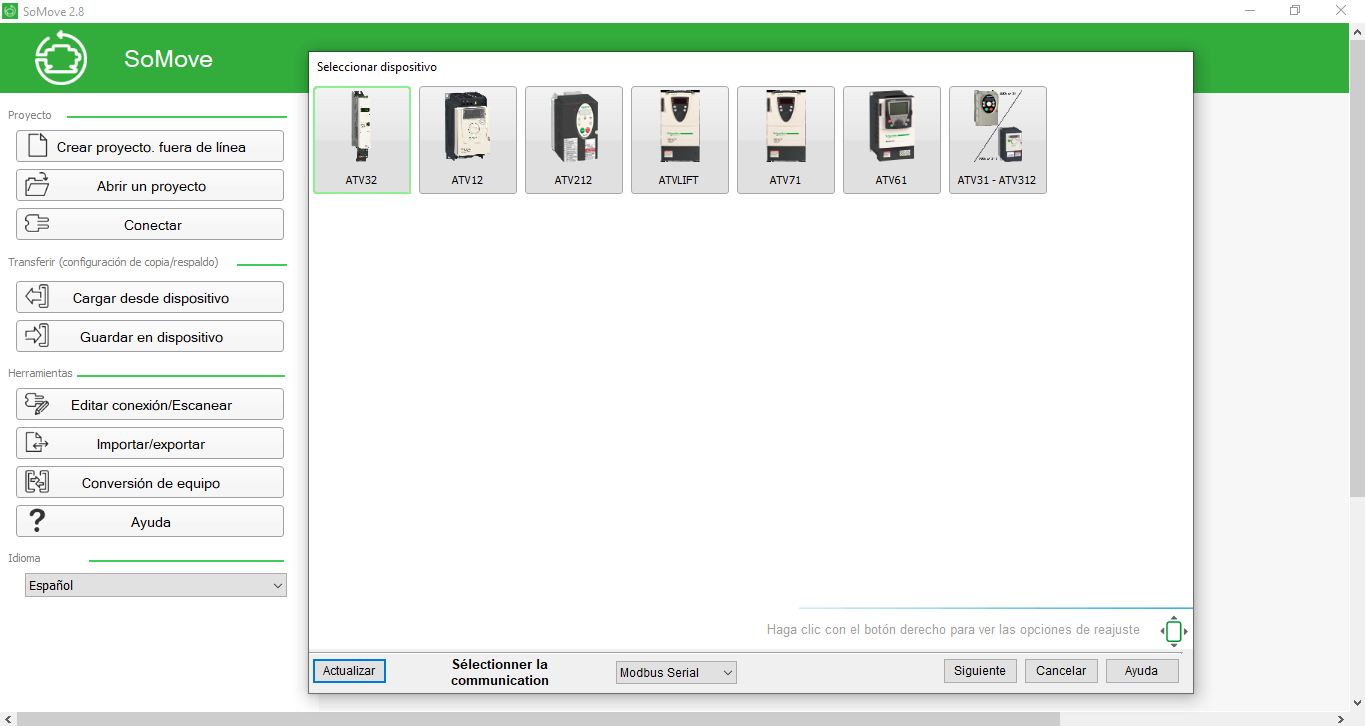
\includegraphics[width=0.9\linewidth]{somove1.png}
	\captionof{figure}{Elección de Altivar 312}
	\label{fig:so1}
\end{figure}
\begin{figure}[H]
	\centering
	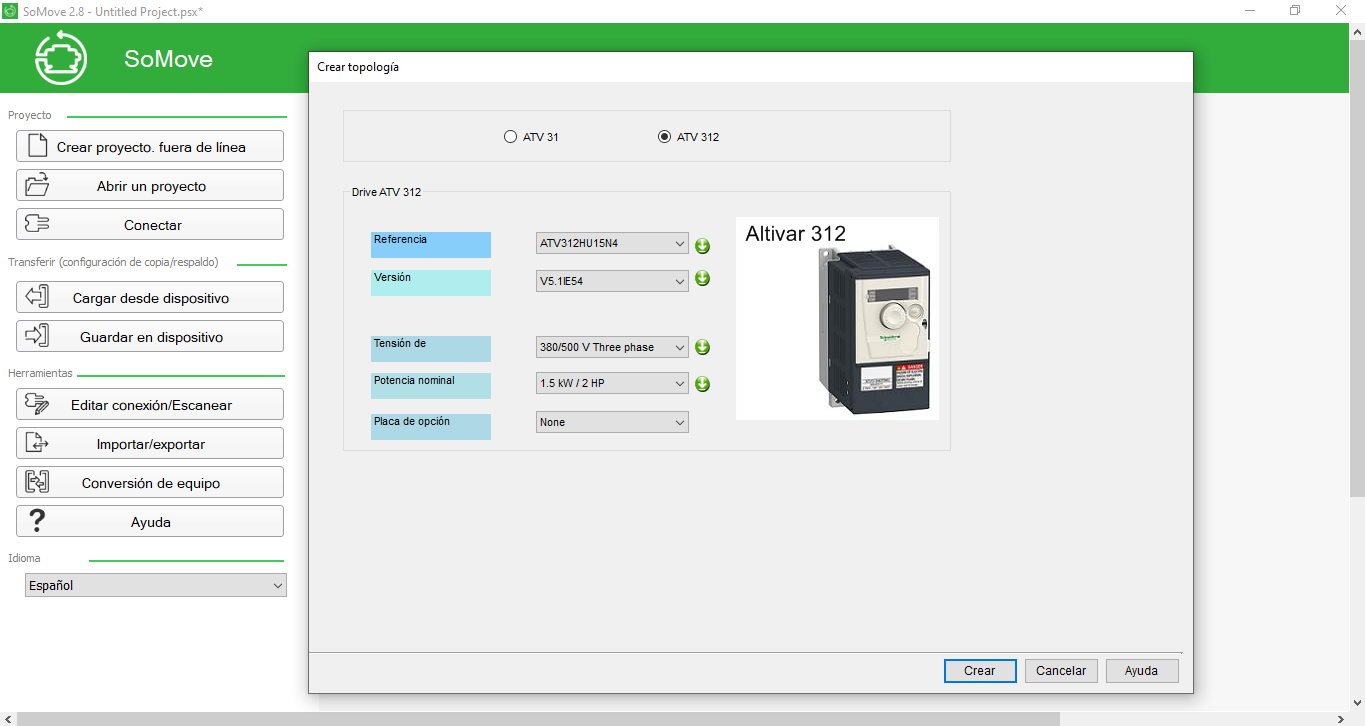
\includegraphics[width=0.9\linewidth]{somove2.png}
	\captionof{figure}{Parámetros del variador}
	\label{fig:so2}
\end{figure}

\begin{figure}[H]
	\centering
	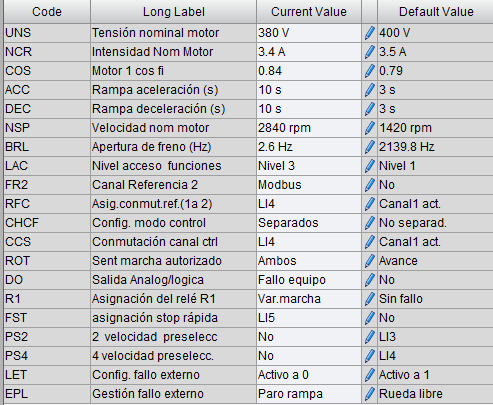
\includegraphics[width=0.9\linewidth]{images/paramsomove}
	\captionof{figure}{Lista de parámetros modificados}
	\label{fig:paramsomove}
\end{figure}


Para realizar esta primera configuración se realizó la comunicación de la computadora con el variador a través del protocolo \textbf{Modbus} (Figura\ref{fig:pcvar}) por medio de un cable que en un extremo poseía una ficha RJ45 con un conversor RS485 y en el otro, ficha USB (Figura \ref{fig:paramsomove1}). 
\begin{figure}[H]
	\centering
	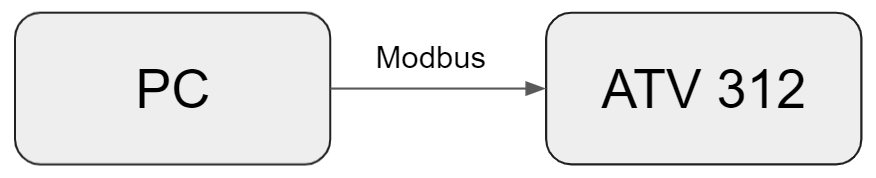
\includegraphics[width=0.7\linewidth]{pc_var.png}
	\captionof{figure}{Diegrama comunicación PC- Variador}
	\label{fig:pcvar}
\end{figure}

\begin{figure}[H]
	\centering
	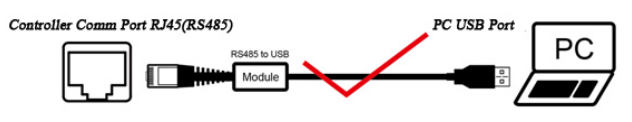
\includegraphics[width=0.9\linewidth]{paramsomove1.png}
	\captionof{figure}{Cable de comunicación}
	\label{fig:paramsomove1}
\end{figure}


\subsection{Comunicación variador de velocidad - PLC}
Para poder realizar la comunicación entre el variador y el PLC es necesario contar con un cable que realice la conexión desde la salida CANOpen a RS485, para esto se necesitó hacer un cable con las fichas correspondientes en cada extremo según las conexiones que muestran en la Figura \ref{fig:cable}, colocando a su vez resistencia de 120 $\Omega$ en cada punta para evitar ruidos eléctricos y fenómenos de reflexión en la línea.

\begin{figure}[htbp]
    \centering
    \subfigure[Ficha entrada/salida variador]{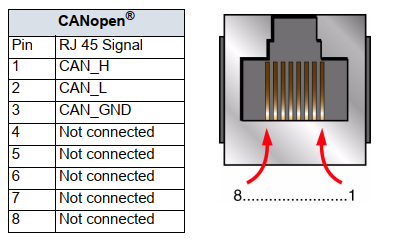
\includegraphics[width=60mm]{canconectores.png}}
    \subfigure[Ficha entrada/salida PLC]{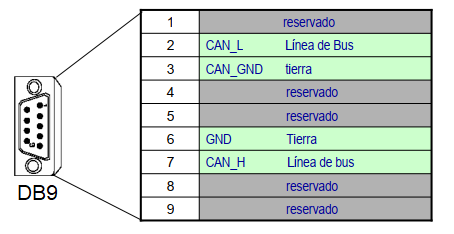
\includegraphics[width=80mm]{candb9.png}}
    \caption{Conexión fichas RJ45- DB9} \label{fig:cable}
    \end{figure}



\subsection{Programación Unity Pro}


Para generar la base del proyecto para trabajar, se debe descargar desde la página oficial e instalar el software Unity Pro XL y la librería DTM utilizada en el software soMove correspondiente al variador que se posee. Una vez que esto está instalado se abre un nuevo proyecto y se configura siguiendo los siguientes pasos.
\begin{enumerate}
	\item Se selecciona el bastidor que se posee.
	\item En la configuración gráfica del bastidor (Figura \ref{fig:uni0})
	podemos introducir los módulos
	deseados haciendo un clic en la
	posición seleccionada (Figura \ref{fig:uni1}).
	El laboratorio cuenta con un PLC modular didáctico de la marca \textbf{Schneider Electric} de la familia \textbf{Modicon} modelo \textbf{M340} con los módulos nombrados anteriormente (Sección \ref{sec:didac}). 
	\item Se debe configurar el módulo Ethernet desde el explorador de
	Proyectos desplegamos la
	carpeta Comunicación y se realiza clic con el botón derecho sobre Redes y luego en Nueva Red, Ethernet (Figura  \ref{fig:inter}).
	\item Se creó una nueva sección para lenguaje FDB para ver parámetros básicos.
	\begin{itemize}
		\item Los Diagramas de Bloques de Función consisten en un Editor gráfico orientado al dibujo
		de bloques. El lenguaje consiste en los Bloques de Funciones reusables elementales y
		derivados.
	\end{itemize}
%\item Para realizar la conexión del PLC con la computadora se utiliza protocolo TCP/IP a través de la dirección 192.168.10.187 (Dirección que el PLC tiene configurada internamente)(Figura \ref{fig:direcc}) y (Figura \ref{fig:inter})
\end{enumerate}
	
	\begin{comment}
	que posee los siguientes módulos:
\begin{itemize}
\item BMX XBP 0400: bastidor para 4 módulos más la fuente de alimentación.
\item BMX P34 2030: CPU 340-20 Ethernet CANopen.   (Comunicación)
\item BMX ART 0414: 4 entradas TC/RTD con separación de potencial.
\item BMX DDM 16022: 8 entradas digitales, y 8 salidas digitales por transistor PNP, todas ellas aisladas.
\item BMX CPS 2000: Fuente de alimentación de 220V
\end{itemize}

	\end{comment}


\begin{center}
	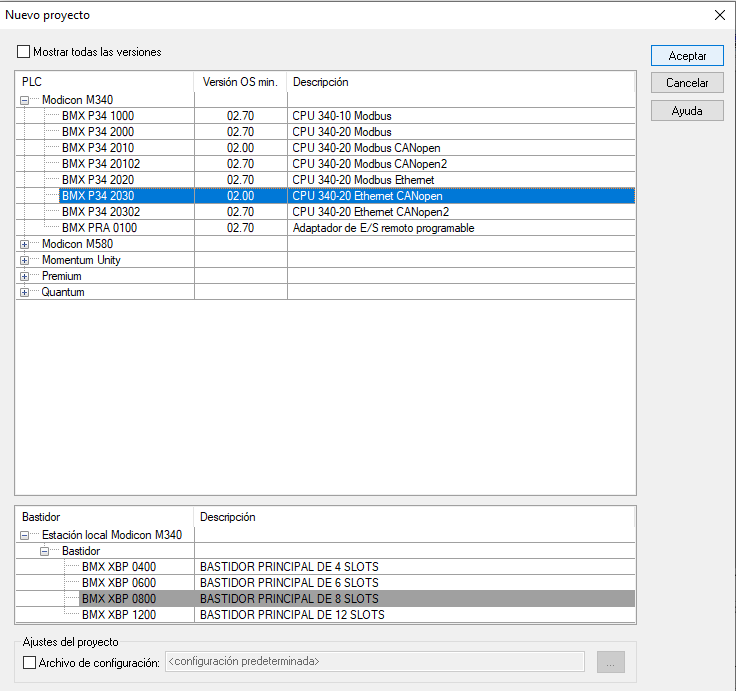
\includegraphics[width=0.9\linewidth]{unit1.png}
	\captionof{figure}{Elección del bastidor}
	\label{fig:uni1}
	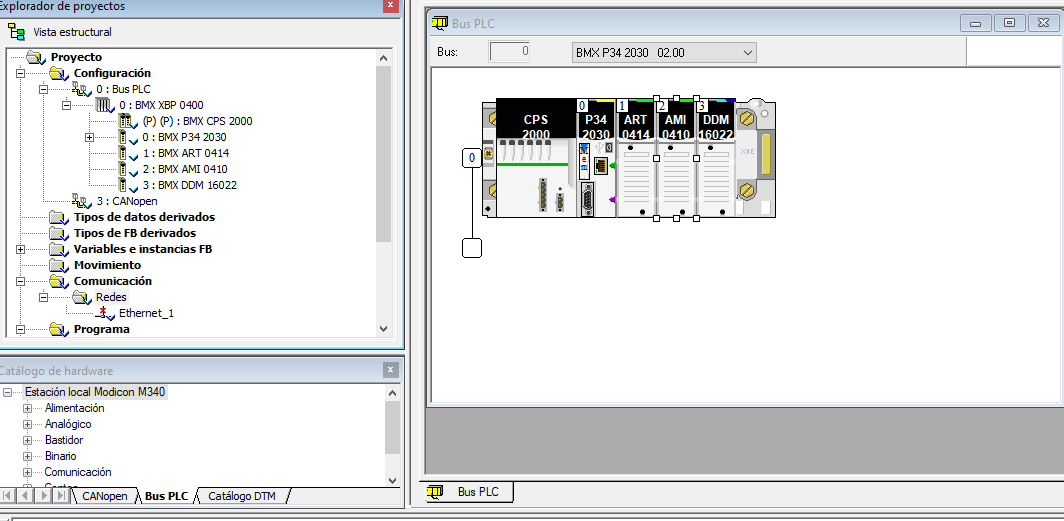
\includegraphics[width=0.9\linewidth]{unity1.png}
	\captionof{figure}{Módulos PLC}
	\label{fig:uni0}
\end{center}

\begin{figure}[h]
	\centering
	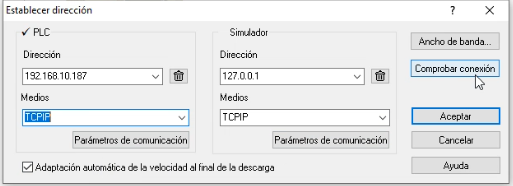
\includegraphics[scale=1]{1.direcc.png}
	\captionof{figure}{Dirección IP}
	\label{fig:direcc}
\end{figure}


\begin{figure}[h]
	\centering
	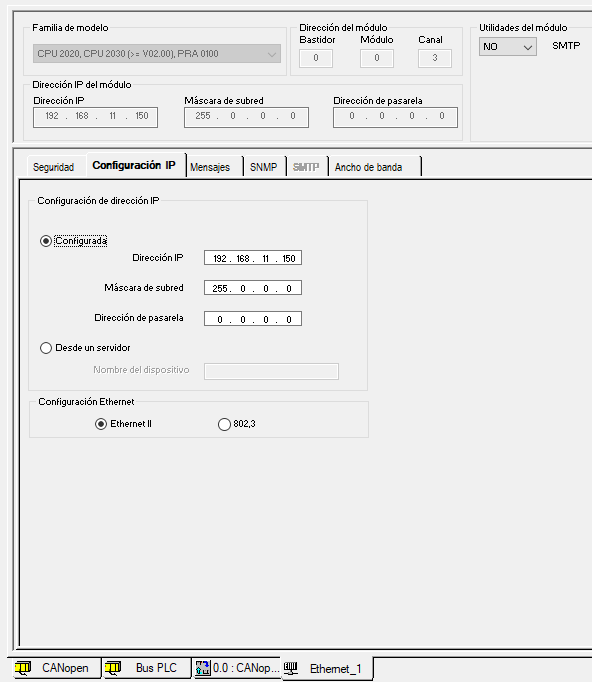
\includegraphics[width=0.9\linewidth]{2.ethern.png}
	\captionof{figure}{Dirección módulo Ethernet}
	\label{fig:inter}
\end{figure}

Una vez que se completó la configuración de la comunicación variador - PLC se procedió a crear una \textit{Pantalla de operador} dentro del mismo programa (Figura \ref{fig:previo})
la cual fue utilizada para interactuar y observar diversos parámetros, como modificar velocidades, observar señales luminosas y ver distintos valores proporcionados por el variador de velocidad.
 
\begin{figure}[H]
	\centering
	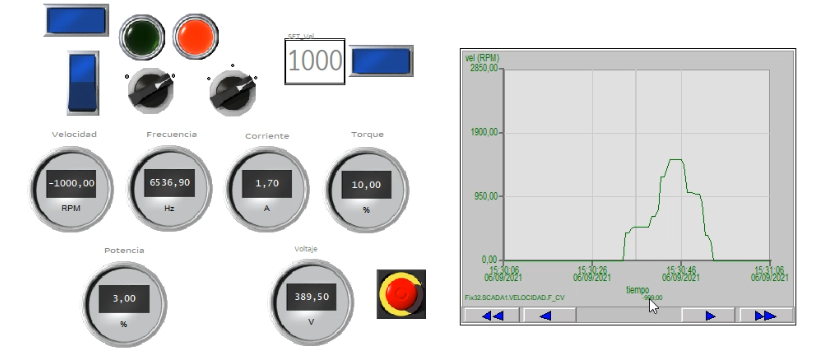
\includegraphics[width=0.9\linewidth]{3.previo.png}
	\captionof{figure}{HMI simple}
	\label{fig:previo}
\end{figure}

Para realizar la programación del HMI se utilizó los bloques de funciones de movimiento (Motion Function Block, MFB) del software UnityPro (Figura \ref{fig:read}). Estos bloques necesitan de un bloque maestro ``CAN\_HANDLER'' el cual permite comprobar la comunicación CANopen, así como la coherencia
entre las configuraciones de software y física.
\\
Otros de los bloques más utilizados dentro del programa fueron ``MC\_READPARAMETER'' que se utiliza para leer, mediante mensajes Service Data Object
(SDO), una variable del variador definida en una dirección CANOpen dada por el fabricante \cite{ComManual}.

\begin{figure}[H]
	\centering
	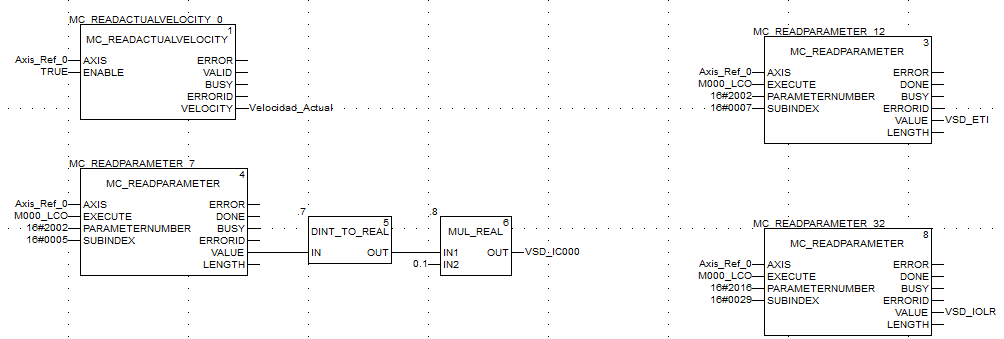
\includegraphics[width=0.9\linewidth]{4.read.png}
	\captionof{figure}{Programa con bloques MFB}
	\label{fig:read}
\end{figure}



\subsubsection{Entradas analógicas}
ESCRIBIR CRISTIAN
\underline{\textit{\textbf{rango-- escalado- 4 a 20mA}}}
\subsubsection{Entradas analógicas TC/RTD}
\textbf{TC/RTD} TERMOCUPLAS RESISTENCIAAAAAAA ??????
ESCRIBIR CRISTIAN




\subsubsection{Medición de caudal}
Según la cantidad de flujo que pase por el caudalímetro, este entregaría pulsos que debían ser leídos con un módulo externo del PLC por la baja resolución que posee. Para esto se planteó utilizar un ESP8266 como interfaz para obtener los pulsos, colocarlos en un registro y enviarlos por un servidor Modbus TCP cada 20ms al PLC. En la sección de programación del PLC se realizó las cuentas correspondientes para realizar la conversión de pulsos a caudal (Figura \ref{fig:modtcp}). Tanto para el módulo, como para el caudalímetro se usó una fuente externa de 3,3 V de alimentación.
\begin{figure}[htbp]
	\centering
	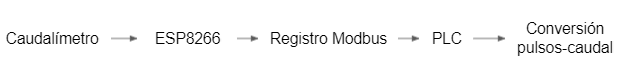
\includegraphics[scale=1]{esp_mod.png}
	\captionof{figure}{Diagrama de flujo del caudalimetro} 
	\label{fig:modtcp}
\end{figure}
\newpage

%\url{
%https://download.schneider-electric.com/files?p_enDocType=User+guide&p_File_Name=35010608_K01_000_11.pdf&p_Doc_Ref=35010608K01000}
